\chapter{RESULTS AND ANALYSIS}
The following report details the training and evaluation of a \gls{lbc} architecture for \gls{hpd}. The model was trained over 45 epochs using a \texttt{OneCycleLR} scheduler before early stopping was triggered.

\section{LBCNN Architecture Performance}
The utilization of \gls{lbc} architecture for the task of human presence detection demonstrated the feasibility of a lightweight model with reliable accuracy on resource-constrained \glspl{mcu}.

\begin{figure}[H]
  \centering
  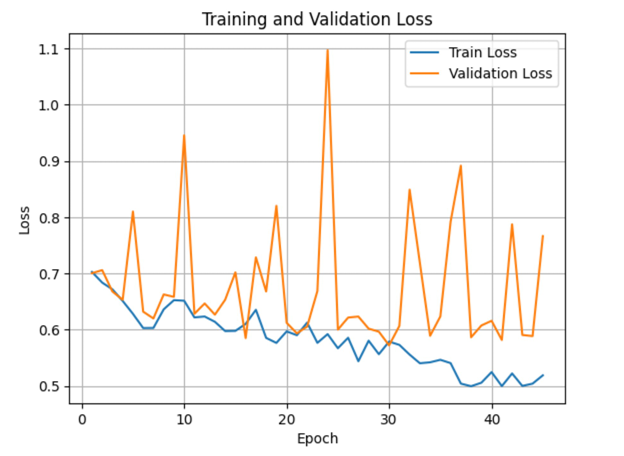
\includegraphics[width=0.85\textwidth]{src/images/1.png}
  \caption{Training and validation loss over 45 epochs.}
  \label{fig:loss_curves}
\end{figure}

The model was trained for 45 epochs (with an early stopping patience of 15) on 737 training samples. As shown in Fig.~\ref{fig:loss_curves}, the training loss decreases consistently while the validation loss remains volatile, indicating moderate overfitting due to the limited dataset size. The best validation loss of \textbf{0.5721} was recorded at epoch 30.

\begin{table}[H]
\renewcommand{\arraystretch}{1.25}
\caption{Training Run Summary}
\label{tab:summary}
\centering
\begin{tabular}{lcc}
\toprule
\textbf{Metric}             & \textbf{Value} & \textbf{Epoch} \\
\midrule
Best validation loss        & 0.5721         & 30             \\
Best validation accuracy    & 77.17\%        & 43             \\
Final training accuracy     & 78.56\%        & 45             \\
Test accuracy               & 71.74\%        & ---            \\
Test \gls{auc} (roc)  & 0.777          & ---            \\
Early stopping              & ---            & 45             \\
\bottomrule
\end{tabular}
\end{table}

\section{Test-Set Evaluation}
Following training, the best-checkpoint model was evaluated on a held-out test set of 92 images. Table~\ref{tab:classification_report} presents the per-class precision, recall, and F1-score.

\begin{table}[H]
\renewcommand{\arraystretch}{1.25}
\caption{Per-Class Classification Report on the Test Set ($n = 92$)}
\label{tab:classification_report}
\centering
\begin{tabular}{lcccc}
\toprule
\textbf{Class}       & \textbf{Precision} & \textbf{Recall}
                      & \textbf{F1-score}  & \textbf{Support} \\
\midrule
Class~0 (No human)   & 0.6190 & 0.7222 & 0.6667 & 36 \\
Class~1 (Human)      & 0.8000 & 0.7143 & 0.7547 & 56 \\
\midrule
Macro average        & 0.7095 & 0.7183 & 0.7107 & 92 \\
Weighted average     & 0.7292 & 0.7174 & 0.7203 & 92 \\
\midrule
\multicolumn{4}{l}{\textbf{Overall test accuracy}} & \textbf{71.74\%} \\
\bottomrule
\end{tabular}
\end{table}

\begin{figure}[H]
  \centering
  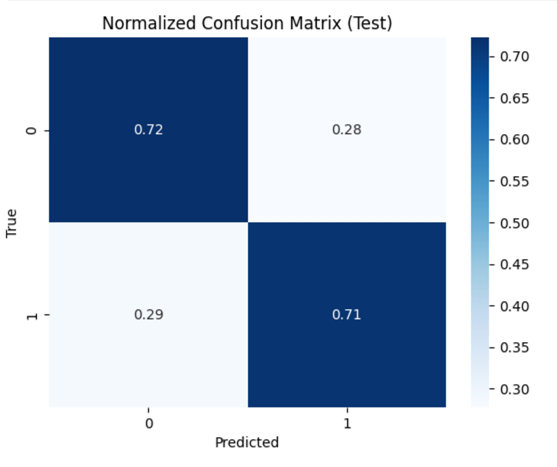
\includegraphics[width=0.75\columnwidth]{src/images/2.png}
  \caption{Normalised confusion matrix on the test set.}
  \label{fig:confusion}
\end{figure}

The model achieves a test accuracy of \textbf{71.74\%} and an \gls{auc} of \textbf{0.777}. As shown in Fig.~\ref{fig:confusion} and Table~\ref{tab:classification_report}, the per-class recall is balanced ($0.72$ and $0.71$), confirming that weighted sampling prevented a majority-class collapse. Notably, Class 1 precision ($0.80$) exceeds Class 0 precision ($0.62$), indicating the model favors human detection—a desirable property for surveillance applications where missed detections are more critical than false alarms.

% \section{Hardware Implementation Analysis}
% The practical deployment utilized a decentralized cluster of ESP32-CAM and \gls{mcu} modules. Initial configuration involved retrieving unique mac addresses to establish a secure communication map. The ESP32-CAM was configured for a resolution of $224 \times 224$ pixels, subsequently partitioned into a $7 \times 7$ grid of $32 \times 32$ pixel tiles.

% \subsection{Saliency Filtering and Communication}
% A key innovation was the use of a Sobel operator to calculate edge density as a Score. This allowed the system to prioritize information-rich regions and ignore redundant background areas. This filtering reduced the data payload by selecting only the top 20 tiles for transmission via the \gls{esp} protocol. While the architecture proved viable, real-world latency was affected by the sequential processing of i2c display updates and the initial Sobel filtering on the input node.